\section{Introducció}

El concepte d'una \emph{màquina pensant} es va introduir el 2500 a.C, quan els egipcis buscaven en estàtues parlants consells místics. Segles després, durant el segle XV, els autòmats preferits de al societat eren els ossos que tocaven tambors i figuretes ballarines que apareixien cada vegada que un rellotge marcava l'hora. \emph{Isaac Asimov}, un símbol en el camp de la robòtica, va ser escriptor, erudit i autor de les lleis de la mateixa. \emph{Asimov} estaba anys llum dels pensadors de l'època i va fer prediccions en les quals la \emph{cibernètica} (a Asimov li agradava referir-se a la robòtica amb el nom de cibernètica), provocaria una revolució intel·lectual. 
Issac Asimov va escriure en el pròleg de \emph{Thinking by Machine: a Study of Cybernetics}, de \emph{Pierre de Latil}:

\begin{quote}
\emph{``La cibernètica no és merament una branca de la ciència, és una revolució intel·lectual que rivalitza en importància la Revolució Industrial. És possible que al igual que una màquina pot fer-se càrrec de les funcions rutinàries dels músculs humans, un altre pugui fer-se càrrec dels usos de rutinaris de la ment humana?''}

\end{quote}

Finalment el terme va ser establert el 1956, en la \emph{Conferència de Darmouth}, un congrés en el qual es van fer previsions triomfalistes a deu anys que mai es van complir, el que va provocar l'abandó gairebé total de les investigacions durant quinze anys. En la \emph{Conferencia de Darmouth} es va intentar esbrinar com fabricar màquines que, utilitzant el llenguatge natural, formessin abstraccions i conceptes, i siguessin capaces d'auto-millorar-se; l'estudi va durar 2 mesos i estava format per 10 persones. El matemàtic, lògic, científic de la computació, criptògraf  i filòsof britànic \emph{Alan Turing} ja havia dissenyat en el 1936-1937 la \emph{Maquina de Turing} (model computacional que va demostrar que no hi ha un mètode definit que es pugui aplicar a qualsevol sentència matemàtica). La pregunta bàsica que Turing va tractar de respondre era \cite{Matur} \cite{Algor}: 

\begin{quote}
	\emph{``Poden les maquines pensar?''}
\end{quote}

Els arguments a favor de Turing sobre la intel·ligència artificial, van iniciar un debat intens que va marcar clarament la primera etapa d'interacció entre la intel·ligència artificial i la psicologia. De fet, se sap que anys enrere diferents filòsofs i matemàtics ja pensaven tant en la intel·ligència artificial com en el seu funcionament; per exemple, Aristòtil, va ser el primer en descriure de manera estructurada un conjunt de regles que descrivien el funcionament de la ment humana \cite{IAgen} \cite{IAgenII}.

\section{Evolució de la IA}

\begin{figure}[ht!]
\centering
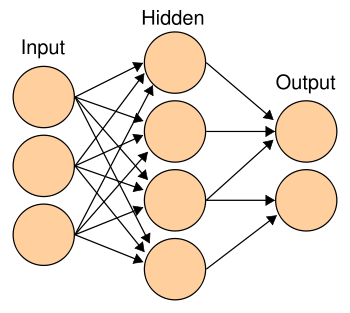
\includegraphics[height=35mm]{data/nn.png}
\caption{Esquema simple d'una xarxa neuronal de topologia 3-4-2.}
\label{nn}
\end{figure} 


\begin{itemize}
\item  \emph{Aristòtil} (300 a.C): va ser el primer en descriure de manera estructurada un conjunt de regles que descrivien el funcionament de la ment humana
\item  \emph{Ctesibi d'Alexandria} (250 a.C): va desenvolupar una màquina capaç de regular el flux d'aigua que actua modificant el comportament de la màquina.
\item \emph{Gottlob Frege} (1879): amplià la lògica booleana i establí la \emph{Lògica del Primer Ordre} (sistema lògic-deductiu que restringeix quines són les expressions correctament formades). Aquesta ordre és tant summament important que té el poder expressiu suficient per definir pràcticament totes les matemàtiques.
\item \emph{Lee De Forest} (1903): inventa el tríode, un component electrònic usat per amplificar, commutar, o modificar una senyal elèctrica. \cite{Tri}
\item \emph{Alan Turing} (1936-1937): considerat com el pare de la ciència informàtica, va formular el concepte de \emph{algorisme}, i va inventar la \emph{Màquina de Turing}. Va ajudar a Anglaterra contra els Alemanys en la Segona Guerra Mundial i va publicar un article on es va demostrar que existeixen problemes dels quals no es pot obtenir una solució; ni per mitjà humà ni per l'ús de computadores.
\item \emph{Warren McCulloch i Walter Pitts} (1943): van formular un model de \emph{neurones artificials} \ref{nn} sense considerar-se un treball del camp de la intel·ligència artificial degut a la inexistència d'aquesta en la època.\cite{EvoIA}
\item \emph{Introducció de la lògica} (1958): en John McCarthy va introduir la lògica en la recerca de la IA, i el 1963, en J. Alan Robinson havia descobert un simple mètode per a implementar la deducció en programes informàtics \cite{machineswhothink}.
\item \emph{Backpropagation} (1982): Rumelhart, Hinton i Williams popularitzen el nou mètode per a entrenar xarxes neuronals \cite{mlintro}, la \emph{propagació marxa enrere}, que s'utilitza avui en dia en molts dels dissenys de xarxes neuronals \cite{mlalgo09}.
\item \emph{Cyc} (1984): s'inicia una base de dades que pretén emmagatzemar els coneixements que tot ésser humà en una cultura moderna té. El projecte es manté actiu avui dia, amb una alternativa lliure, \emph{OpenCyc} \cite{opencyc}.
\item \emph{Deep Blue} (1997): super-ordinador que va guanyar al campió d'escacs Garry Kasparov \cite{deepblue}.
\item \emph{Watson} (2011): super-ordinador que va guanyar als dos millors participants del programa nord-americà \emph{Jeopardy!} \cite{watsonjeopardy}.
\end{itemize}

\section{El test de Turing}

\emph{Alan Turing}, va dissenyar un simple i lògic model matemàtic durant 1950 capaç de \emph{verificar si una màquina és o no intel·ligent}.

El test és duu a terme simplement situant un humà i una màquina separats per una paret. El test es basarà en l'humà, que haurà de anar formulant preguntes i la màquina les haurà de respondre. L'humà, al ser inconscient de que està parlant amb una màquina, haurà de jutjar si les respostes que rep són lògiques, o no. Si creu que ho són, es considerarà que la màquina en qüestió és intel·ligent. \cite{Matur}
